\chapter{Authentication Mechanisms}
\label{cha:authentication_mechanisms}
This chapter explains the concepts and mechanisms of the discussed authentication mechanisms.
Only the mTLS and and the JWT approach are discussed, since the TTN approach is deprecated and should not be used anymore~\cite{dias2020microservices}.
Furthermore this chapter clarifies the advantages and disadvantages of the discussed mechanisms.

\section{Authentication based on mTLS}
Mutual TLS is the most popular option for the service-to-service authentication of microservice deployments~\cite{dias2020microservices}.
Securing the communication with TLS already provides integrity, confidentiality and furthermore authenticates the server to the client.
Since basic TLS does not provide authentication from the client to the server, it is not sufficient for the service-to-service security.
Therefore mutual TLS is used, which provides an efficient and straightforward approach to authenticate the client to the server.

% TODO: Find better title for this subsection
\subsection{General}
The authentication using mTLS requires a PKI, same as the authentication using basic TLS.
It is possible to use the already existing PKI of the internet, but this would make the key management much harder and would bring no advantages.
% TODO: Insert Reference to self hosted PKI
Therefore it is good practise to use a self-hosted PKI to have a root of trust within the network~\cite{dias2020microservices}.
The setup of a microservice deployment using mTLS is shown in figure~\ref{fig:auth_mechanisms_mtls}.

When mTLS is used, both the server and the client must provide a valid certificate to create a communication channel.
The issuer of the presented certificates must be trusted by all communicating parties~\cite{dias2020microservices}.
If one communication partner does not have a valid certificate which is signed by a trusted issuer, the communication is neglected.
Therefore each service needs a private key, a public key and a signed certificate, which binds the public key to the subject of the certificate, which is the service.
The certificates of the communication partners are exchanged during the TLS handshake.
The server presents his certificate to the client after he receives the helo message of the client.
And the client presents his certificate to the server, together with the pre-master secret~\cite{krawczyk2013security}.

\begin{figure}
	\centering
	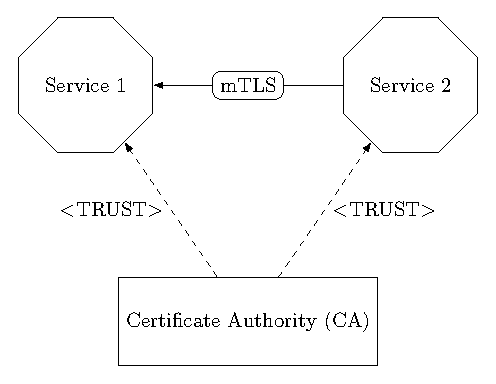
\includegraphics{images/authentication-mechanisms/TikZ_mTLS_base_structure.pdf}
	\caption{Setup using mTLS for the service-to-service authentication~\cite{dias2020microservices}}
	\label{fig:auth_mechanisms_mtls}
\end{figure}

